\documentclass[11pt]{article}
\usepackage[a4paper, margin=2.54cm]{geometry}
\usepackage[utf8]{inputenc}
\usepackage[spanish]{babel}
\usepackage[spanish]{layout}
\usepackage[article]{ragged2e}
\usepackage{textcomp}
\usepackage{caption}
\usepackage{subcaption}
\usepackage{graphicx}
\usepackage{multirow}

% ============================================================================
% ============================================================================
% ============================================================================

\title{
  TRABAJO PRÁCTICO N° 1\\
  \large Estado de la arboleda en el sur de Buenos Aires
}
\author{
  Farizano, Juan Ignacio\\
  \and
  Mellino, Natalia
}
\date{}

% ============================================================================
% ============================================================================
% ============================================================================

\begin{document}

\maketitle
\newpage

\tableofcontents
\newpage

% ============================================================================
% ============================================================================
% ============================================================================

\section{Introducción}
\textbf{Motivación del problema:}

\begin{justify}
  En el año 2011 se realizó un Censo Forestal Urbano Público en dos
  comunas del sur de Buenos Aires y esta será nuestra fuente de información
  a lo largo del informe.
  En éste analizaremos los datos de dicho censo con el objetivo
  de determinar el estado actual del arbolado urbano público.\\
  Las variables incluidas en la base de datos dada se describen a continuación.
\end{justify}

% Tabla de variables
\begin{center}
  \begin{tabular}{| c | p{9cm} | c |}
    \hline
    \textbf{Nombre} & \textbf{Descripción} & \textbf{Tipo de variable} \\ \hline
    ID & Identificación del árbol. & - \\ \hline
    Altura & Altura de cada árbol, medida en metros (m). Observación: si un árbol
    mide 12,7 m se tomará como dato “12”, truncando los valores a la unidad. & 
    Cuantitativa continua \\ \hline
    Diámetro & Diámetro de cada árbol, medido en centímetros (cm). & 
    Cuantitativa continua \\ \hline
    Inclinación & Ángulo que forma el tronco del árbol respecto
    a una perpendicular al suelo, medido en grados (°).
    Indica el grado de inclinación del árbol. & Cuantitativa continua \\ \hline
    Especie & Especie a la que pertenece el árbol, dentro de las siguientes
    categorías: Eucalipto, Jacarandá, Palo Borracho, Casuarina, Fresno, Ceibo,
    Ficus, Álamo, Acacia. & Cualitativa nominal \\ \hline
    Origen & Procedencia de la especie: Exótico, Nativo/Autóctono, 
    No Determinado. & Cualitativa nominal \\ \hline
    Brotes & Número de brotes jóvenes crecidos durante el último año. &
    Cuantitativa discreta \\ \hline
  \end{tabular}
\end{center}

% ============================================================================
% ============================================================================
% ============================================================================

\newpage
\section{Análisis univariado}

\subsection{Altura}

\begin{table}[h!]
  \begin{center}
    \begin{tabular}{| c | r | r | r | r |}
      \hline
      \multirow{3}{3cm}{\centering\textbf{Intervalos (altura en m)}} & 
      \multirow{3}{3cm}{\centering\textbf{Frecuencia absoluta}} & 
      \multirow{3}{3cm}{\centering\textbf{Frecuencia absoluta acumulada}} &
      \multirow{3}{3cm}{\centering\textbf{Frecuencia relativa}} & 
      \multirow{3}{3cm}{\centering\textbf{Frecuencia relativa acumulada}} \\
      & & & & \\
      & & & & \\ \hline
      (0,5] & 34 & 34 & 0.0971 & 0.0971 \\ \hline
      (5,10] & 79 & 113 & 0.2257 & 0.3229 \\ \hline
      (10,15] & 92 & 205 & 0.2629 & 0.5857 \\ \hline
      (15,20] & 84 & 289 & 0.2400 & 0.8257 \\ \hline
      (20,25] & 53 & 342 & 0.1514 & 0.9771 \\ \hline
      (25,30] & 5 & 347 & 0.0143 & 0.9914 \\ \hline
      (30,35] & 3 & 350 & 0.0086 & 1.0000 \\ \hline
    \end{tabular}
    \caption{Tabla de frecuencias.}
    \label{tab:tablaAltura}
  \end{center}
\end{table}

\begin{figure}[h!]
  \begin{center}
    \begin{subfigure}[b]{0.9\linewidth}
      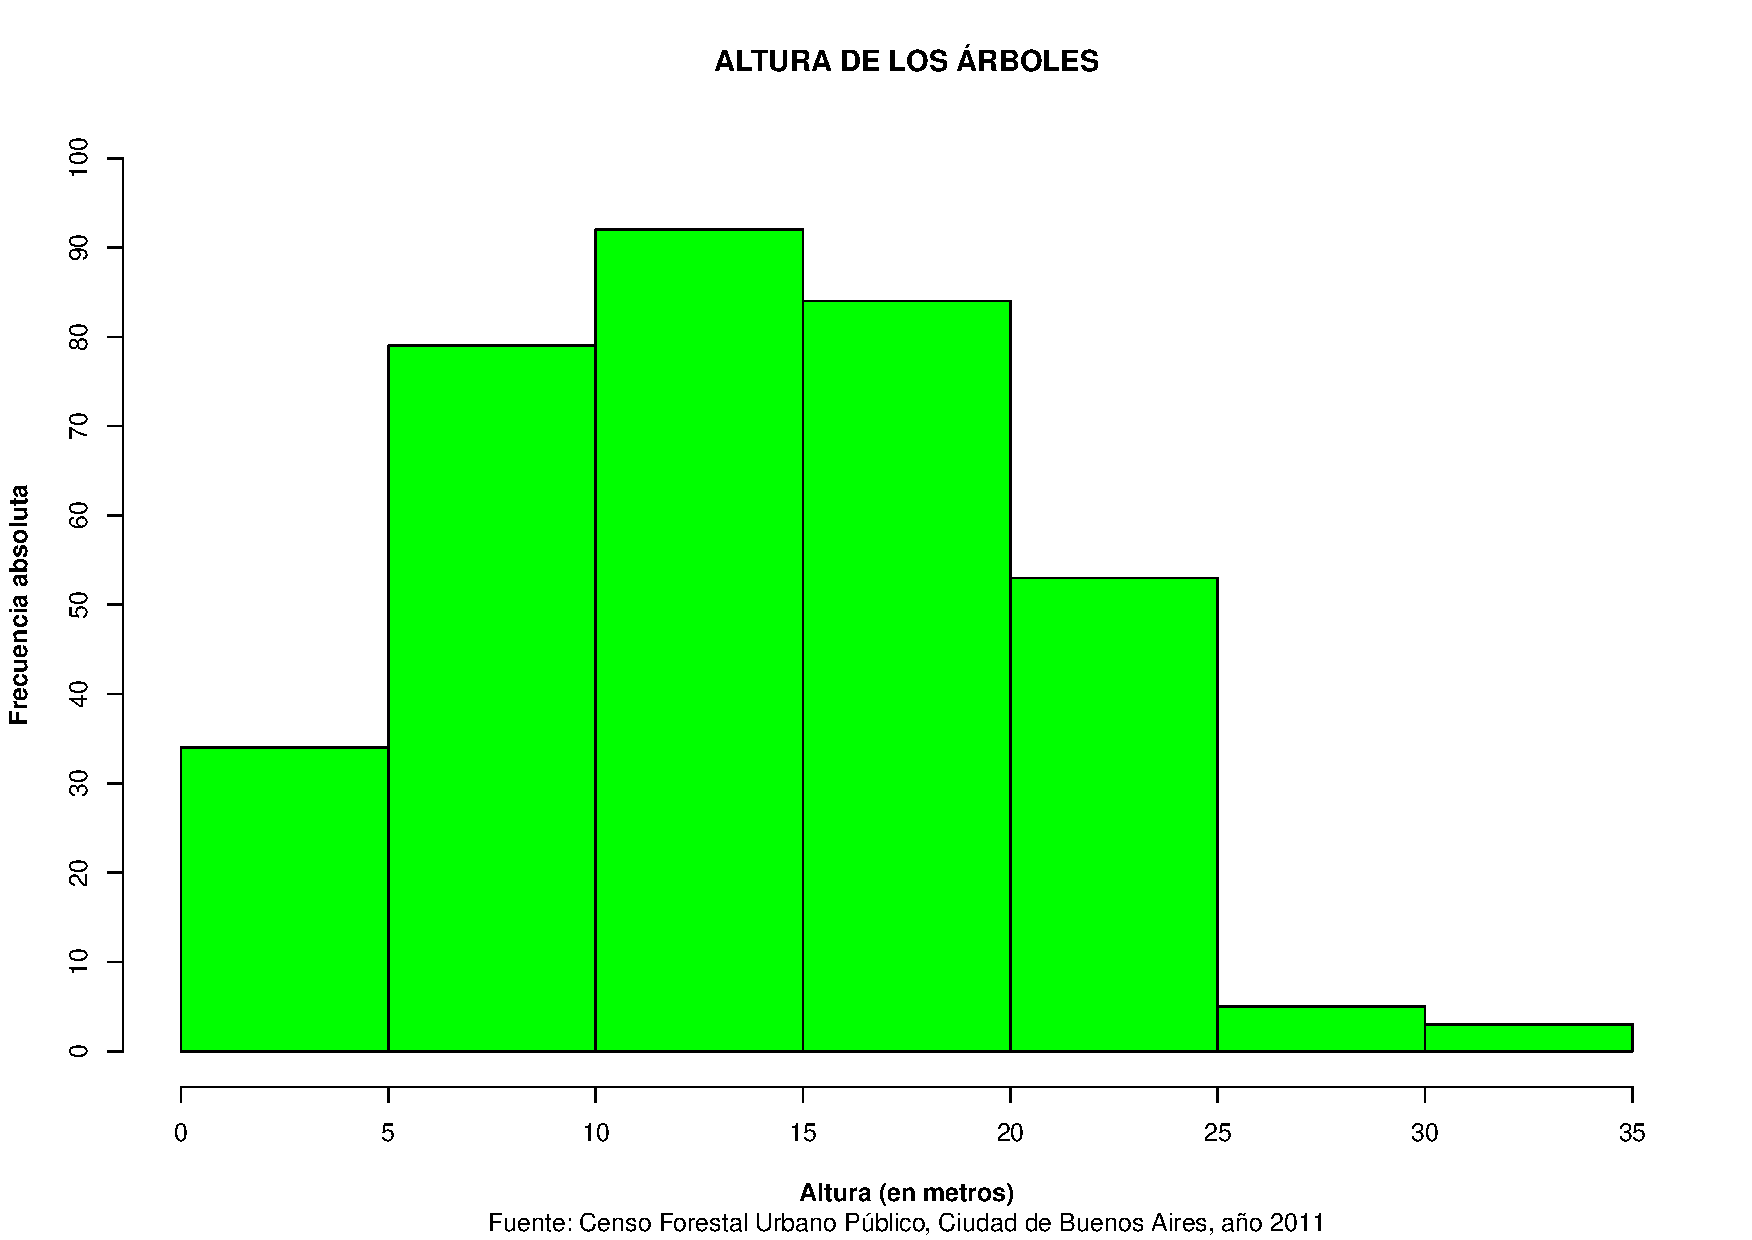
\includegraphics[width=\linewidth]{histAltura.pdf}
      \caption{Histograma.}
      \label{fig:histAltura}
    \end{subfigure}
  \end{center}
\end{figure}

\newpage

\begin{figure}[h!]
  \ContinuedFloat
  \begin{center}
    \begin{subfigure}[b]{0.9\linewidth}
      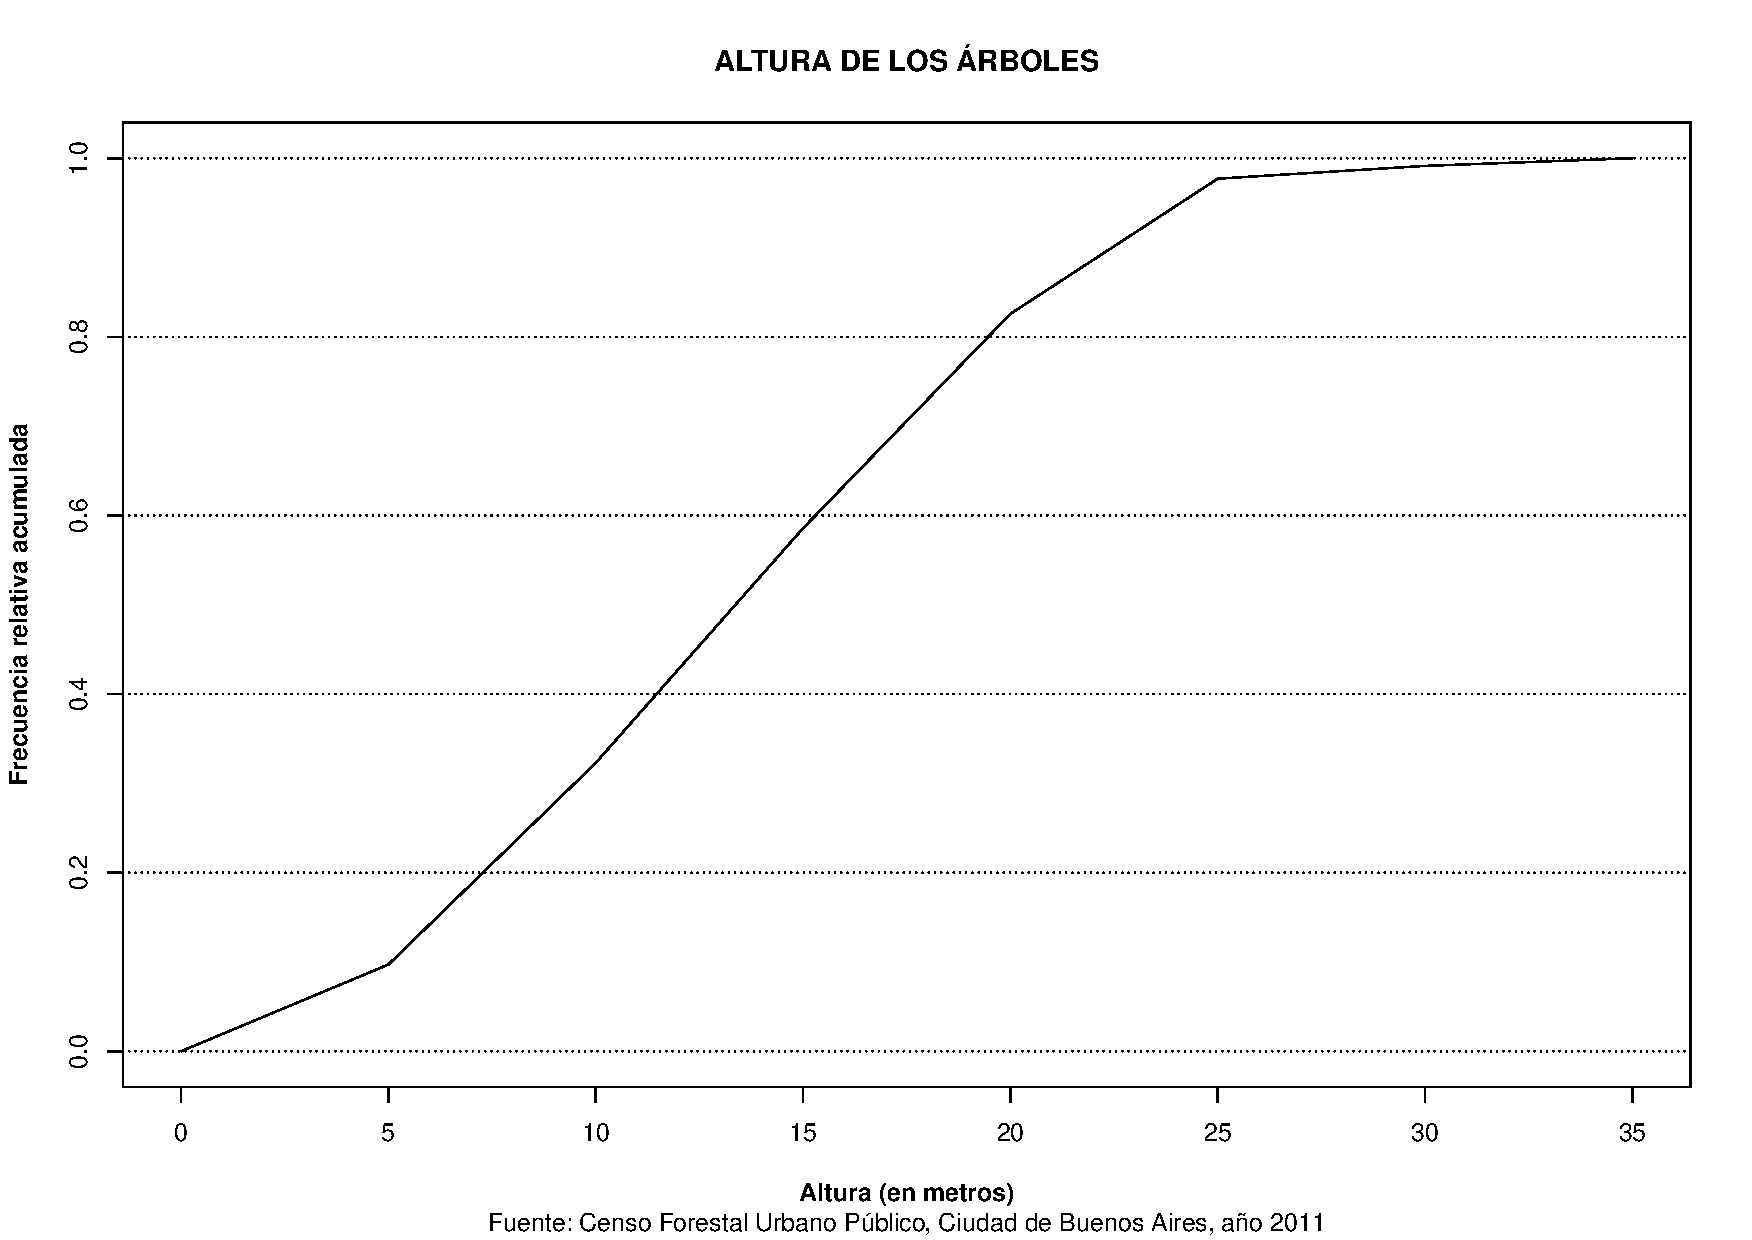
\includegraphics[width=\linewidth]{acumAltura.pdf}
      \caption{Polígono acumulativo.}
      \label{fig:acumAltura}
    \end{subfigure}
  \caption{}
  \end{center}  
\end{figure}

\begin{justify}
  El gráfico \ref{fig:histAltura} es unimodal y asimétrico hacia la derecha,
  donde se puede observar
  que una mayor cantidad de árboles tienen una altura entre 10 y 15 mts.
  Si se observa el polígono acumulativo de la figura \ref{fig:acumAltura} 
  junto con la tabla \ref{tab:tablaAltura} se puede ver que aproximadamente
  el 97\% de la arboleda presenta una altura inferior a 25 mts.
  La altura promedio es de 14.02mts.
\end{justify}

% ============================================================================

\subsection{Diámetro}

\begin{table}[h!]
  \begin{center}
    \begin{tabular}{| c | r | r | r | r |}
      \hline
      \multirow{3}{3cm}{\centering\textbf{Intervalos (diámetro en cm)}} & 
      \multirow{3}{3cm}{\centering\textbf{Frecuencia absoluta}} & 
      \multirow{3}{3cm}{\centering\textbf{Frecuencia absoluta acumulada}} &
      \multirow{3}{3cm}{\centering\textbf{Frecuencia relativa}} & 
      \multirow{3}{3cm}{\centering\textbf{Frecuencia relativa acumulada}} \\
      & & & & \\
      & & & & \\ \hline
      (0,20] & 83 & 83 & 0.2371 & 0.2371 \\ \hline
      (20,40] & 147 & 230 & 0.4200 & 0.6571 \\ \hline
      (40,60] & 69 & 299 & 0.1971 & 0.8543 \\ \hline
      (60,80] & 35 & 334 & 0.1000 & 0.9543 \\ \hline
      (80,100] & 12 & 346 & 0.0343 & 0.9886 \\ \hline
      (100,120] & 2 & 348 & 0.0057 & 0.9943 \\ \hline
      (120,140] & 2 & 350 & 0.0057 & 1.0000 \\ \hline
    \end{tabular}
    \caption{Tabla de frecuencias.}
    \label{tab:tablaDiametro}
  \end{center}
\end{table}

\newpage

\begin{figure}[h!]
  \begin{center}
    \begin{subfigure}[b]{0.9\linewidth}
      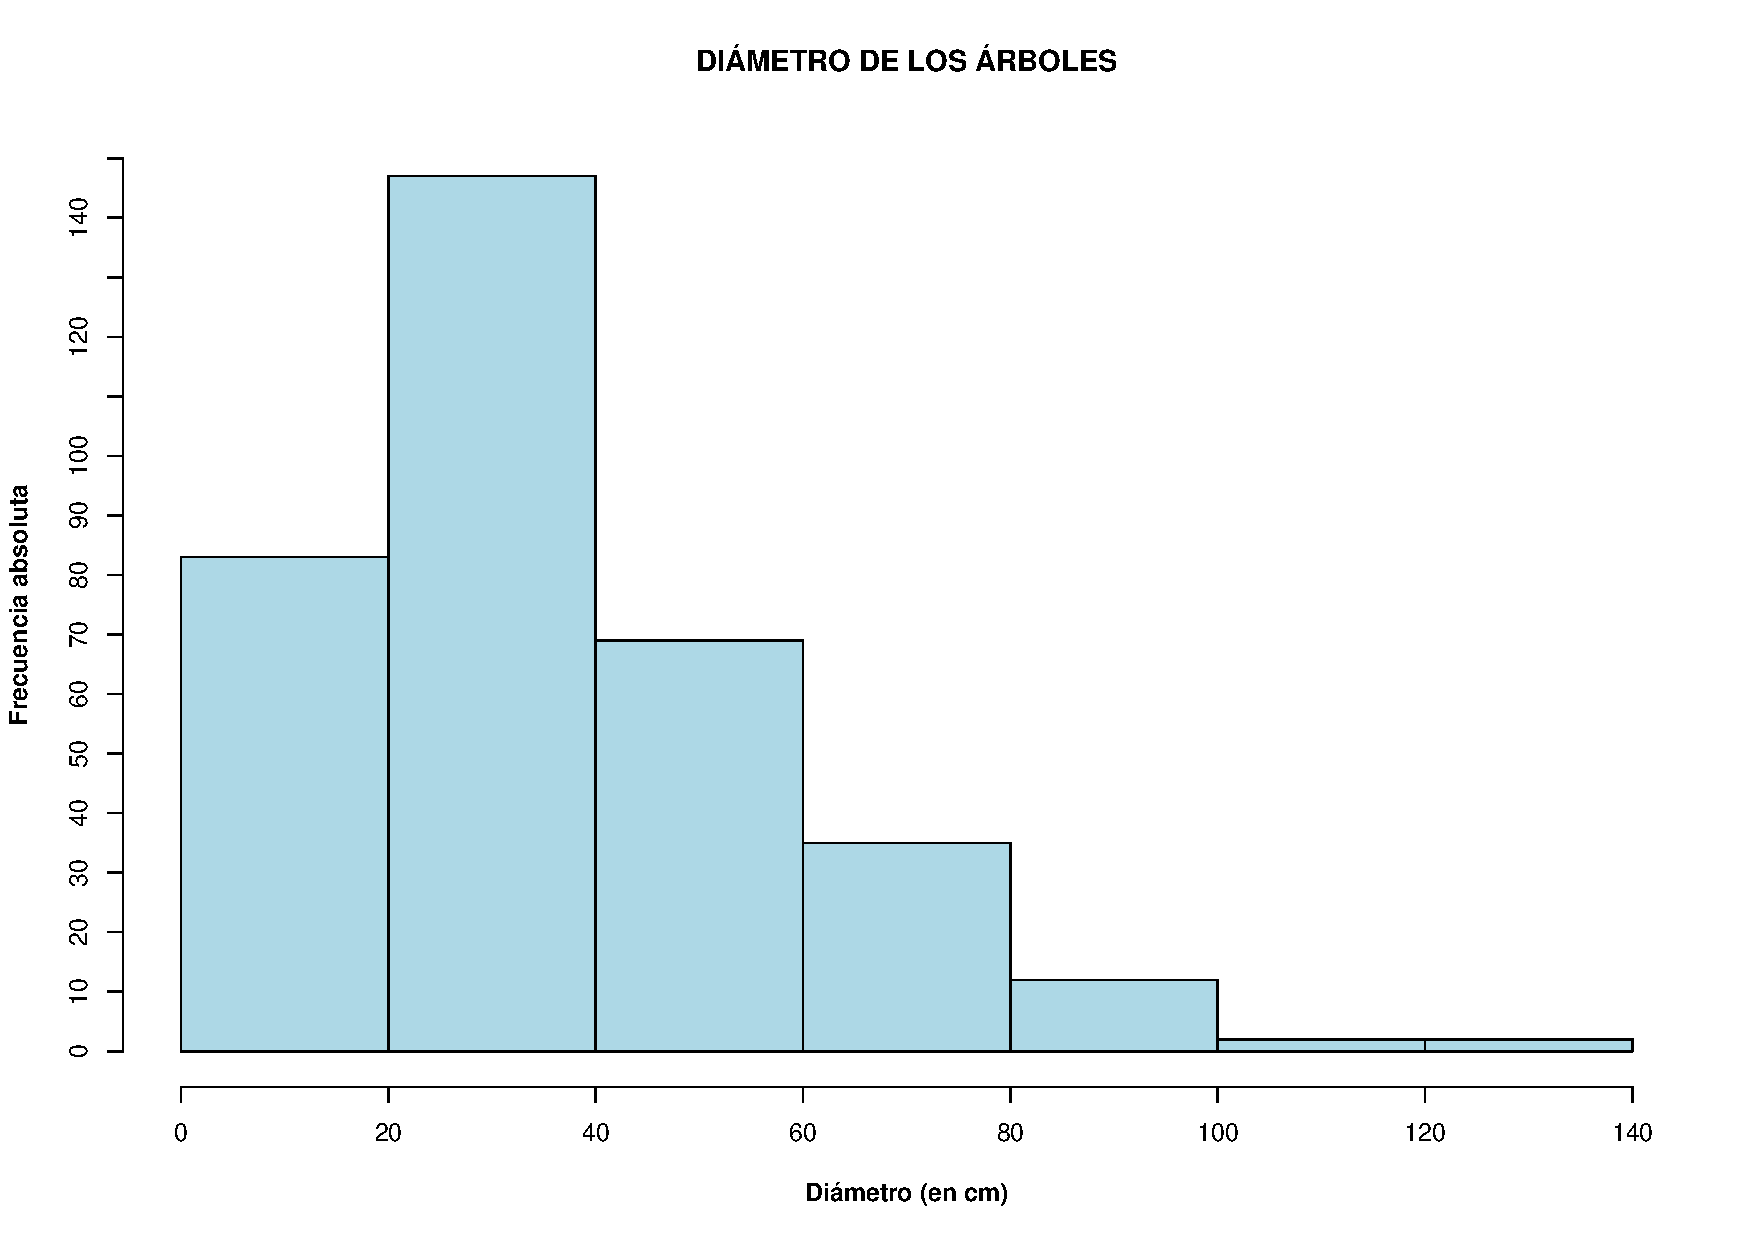
\includegraphics[width=\linewidth]{histDiametro.pdf}
      \caption{Histograma.}
      \label{fig:histDiametro}
    \end{subfigure}
  \end{center}
\end{figure}

\begin{figure}[h!]
  \ContinuedFloat
  \begin{center}
    \begin{subfigure}[b]{0.9\linewidth}
      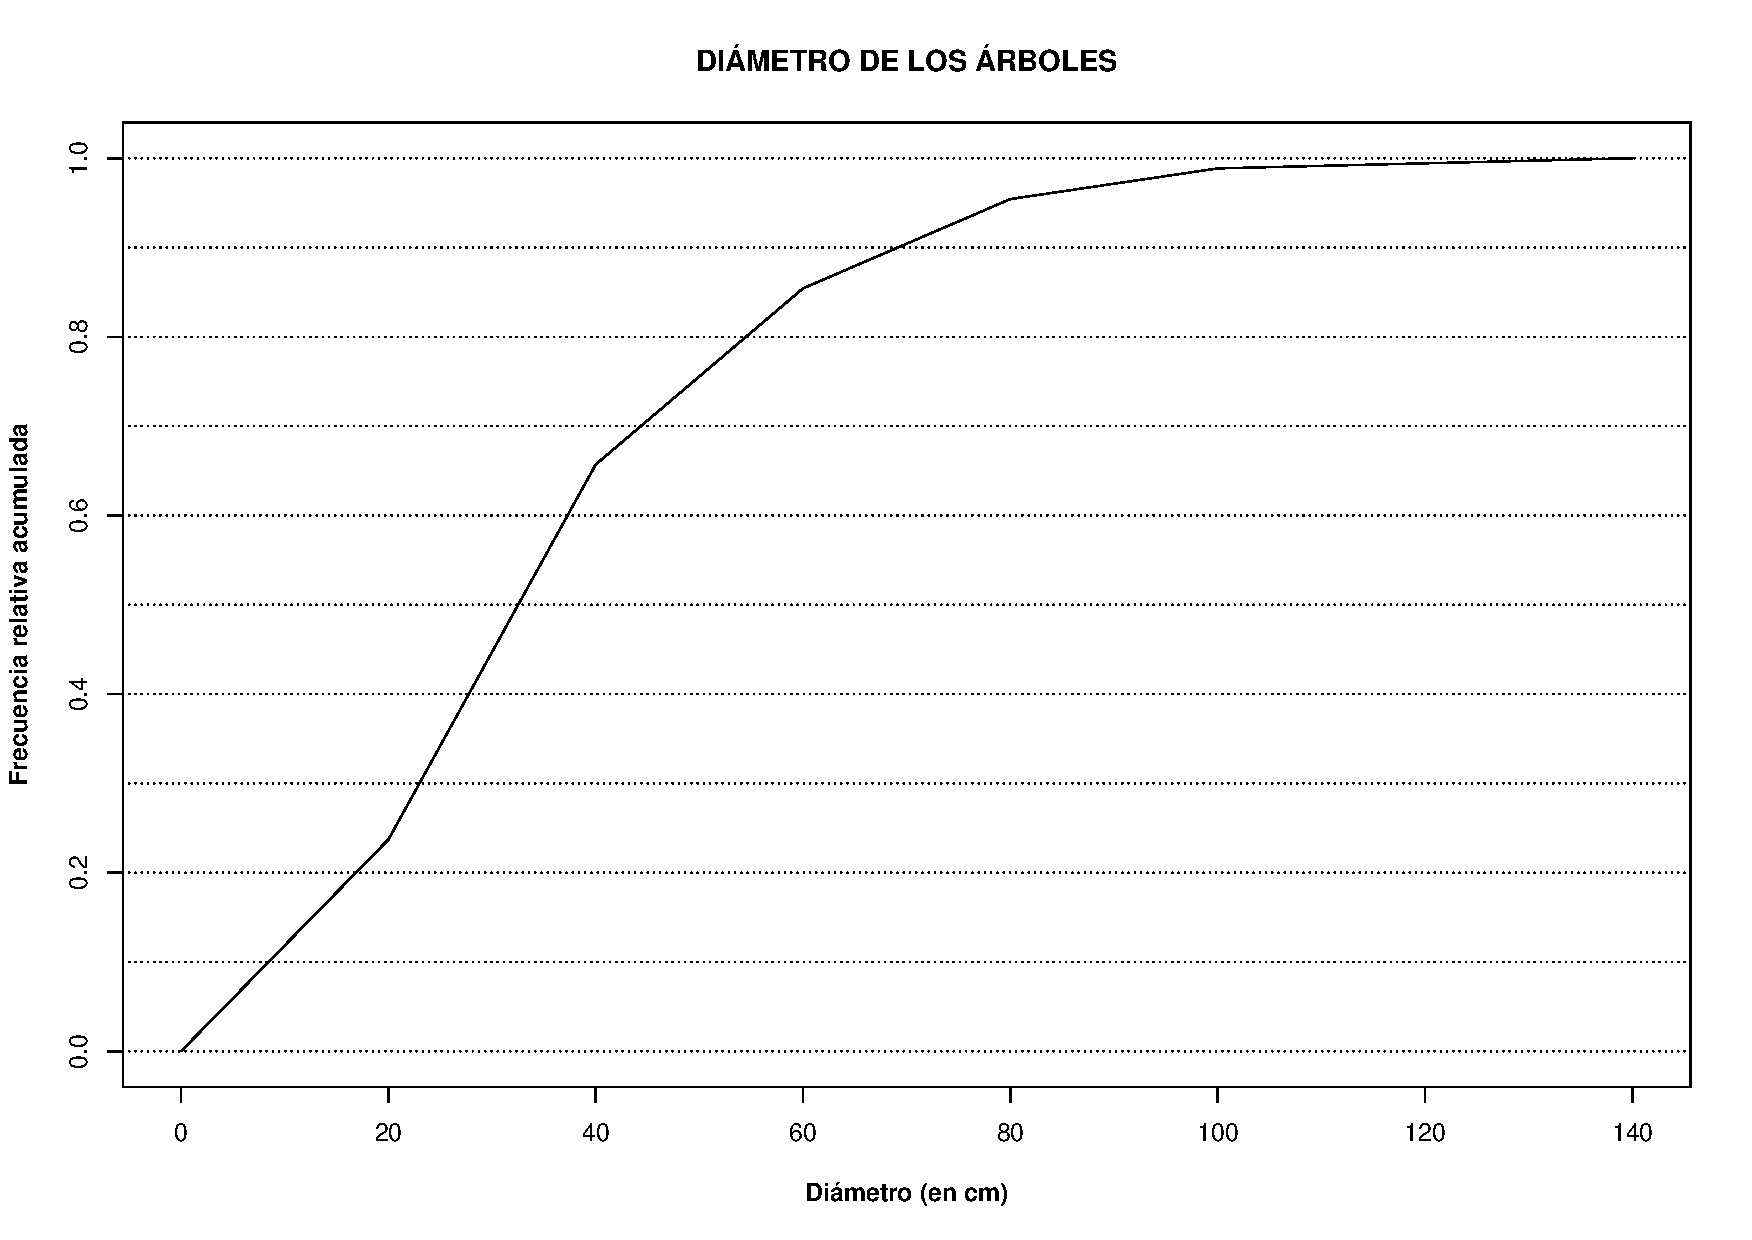
\includegraphics[width=\linewidth]{acumDiametro.pdf}
      \caption{Polígono acumulativo.}
      \label{fig:acumDiametro}
    \end{subfigure}
  \caption{}
  \end{center}  
\end{figure}

\begin{justify}
  Como se puede observar en el histograma de la figura \ref{fig:histDiametro}, 
  éste es asimétrico a la derecha, mostrando una mayor cantidad de árboles que
  poseen un diámetro de entre 20 y 40 cm. El diámetro promedio resultó ser 
  de 37.61 cm. Observando el polígono acumulativo de la figura
  \ref{fig:acumDiametro} se puede comprobar que aproximadamente el 80\%
  de los árboles tienen un diámetro menor a 60cm.
\end{justify}

% ============================================================================

\subsection{Inclinación}

\begin{table}[h!]
  \begin{center}
    \begin{tabular}{| c | r | r | r | r |}
      \hline
      \multirow{3}{3cm}{\centering\textbf{Intervalos (inclinación en grados)}} & 
      \multirow{3}{3cm}{\centering\textbf{Frecuencia absoluta}} & 
      \multirow{3}{3cm}{\centering\textbf{Frecuencia absoluta acumulada}} &
      \multirow{3}{3cm}{\centering\textbf{Frecuencia relativa}} & 
      \multirow{3}{3cm}{\centering\textbf{Frecuencia relativa acumulada}} \\
      & & & & \\
      & & & & \\ \hline
      [0,7) & 294 & 294 & 0.8400 & 0.8400 \\ \hline
      [7,14) & 34 & 328 & 0.0971 & 0.9371 \\ \hline
      [14,21) & 13 & 341 & 0.0371 & 0.9743 \\ \hline
      [21,28) & 4 & 345 & 0.0114 & 0.9857 \\ \hline
      [28,35) & 2 & 347 & 0.0057 & 0.9914 \\ \hline
      [35,42) & 3 & 350 & 0.0086 & 1.0000 \\ \hline
    \end{tabular}
    \caption{Tabla de frecuencias.}
    \label{tab:tablaInclinacion}
  \end{center}
\end{table}

\begin{figure}[h!]
  \begin{center}
    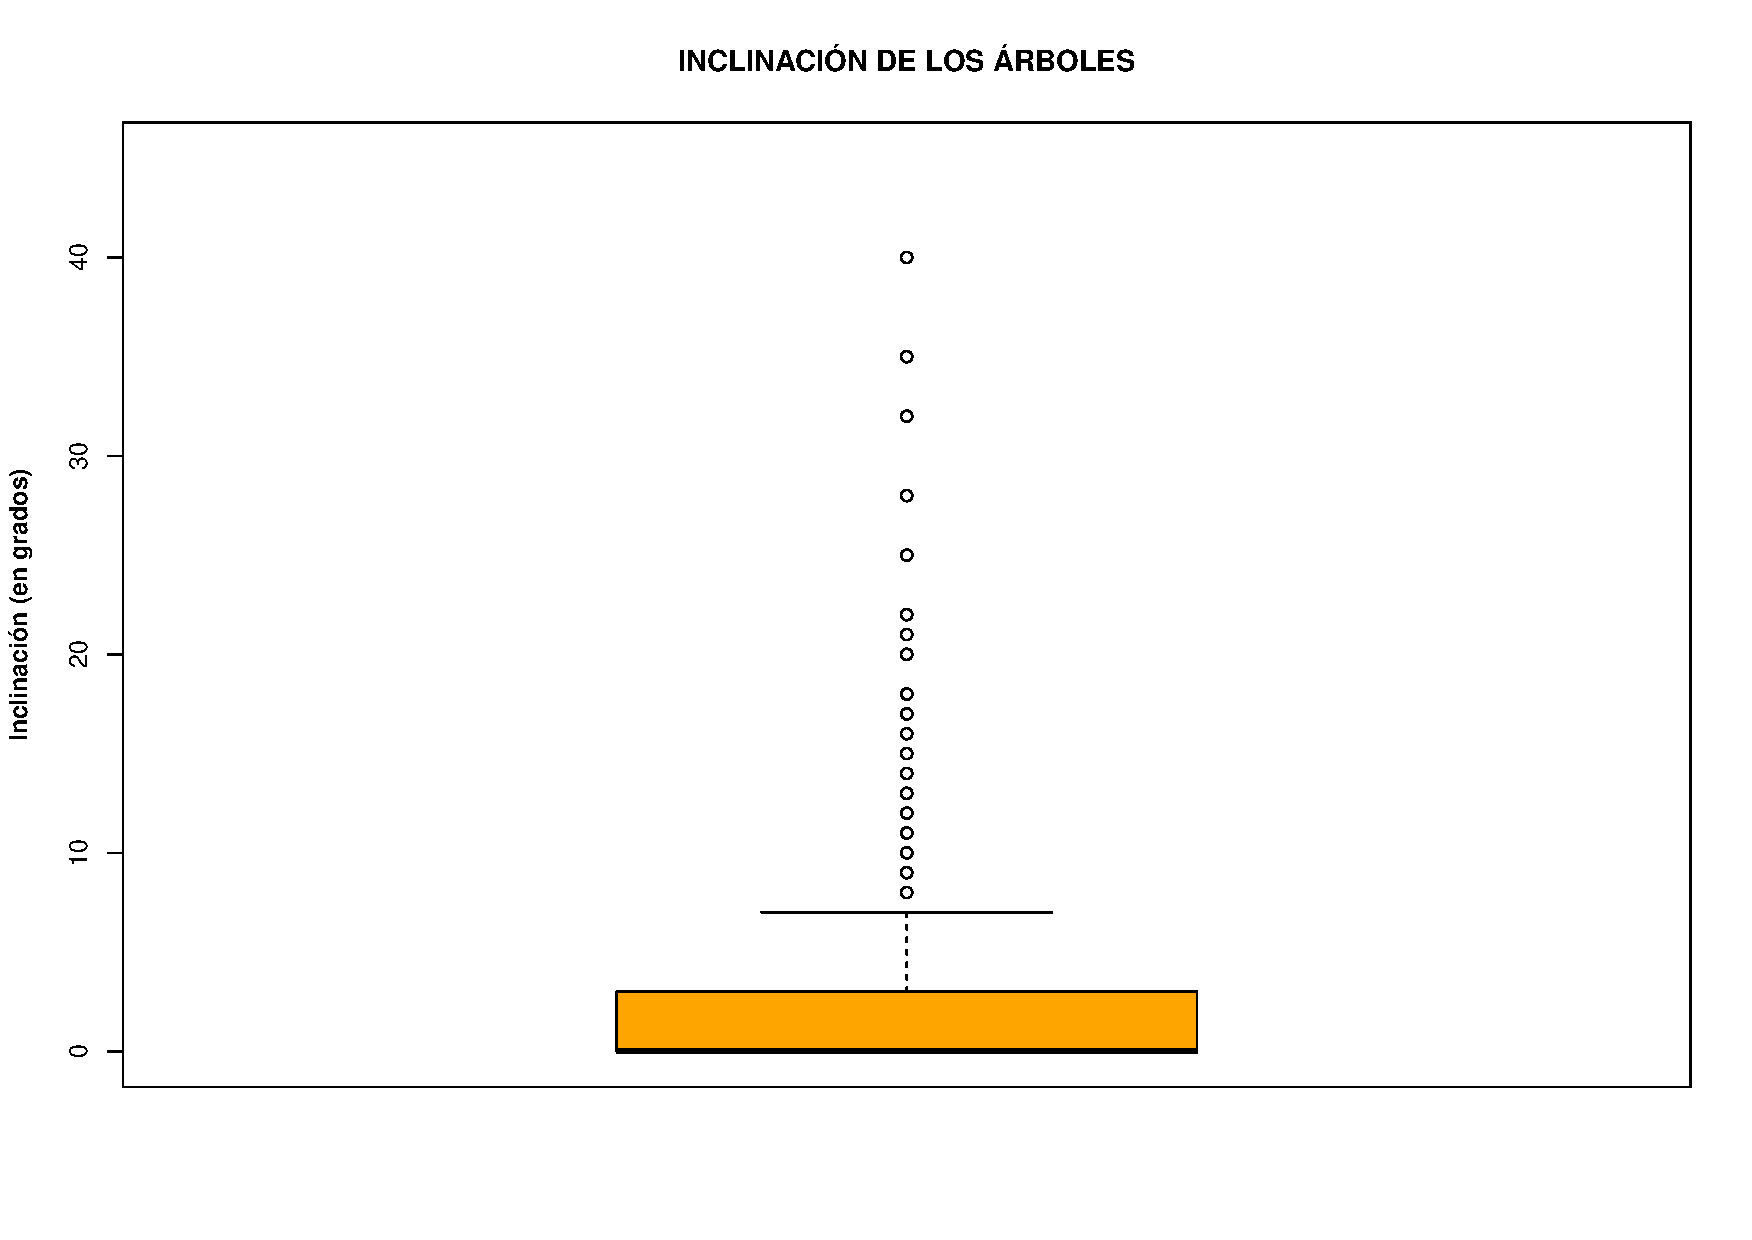
\includegraphics[width=0.9\linewidth]{boxInclinacion.pdf}
    \caption{Gráfico de caja.}
    \label{fig:boxInclinacion}
  \end{center}  
\end{figure}

\begin{justify}
  En el gráfico de caja \ref{fig:boxInclinacion} se observa que la mediana
  es de 0 grados, siendo que aproximadamente el 73\% de los árboles tienen
  esta inclinación, y además observando la tabla \ref{tab:tablaInclinacion}
  se ve que los valores adyacentes que van de una inclinación de 0 a 7 grados
  componen el 84\% de la arboleda. Fuera de este rango, se encuentran
  52 observaciones outliers. 
\end{justify}

% ============================================================================

\subsection{Especie}

\begin{table}[h!]
  \begin{center}
    \begin{tabular}{| c | r |}
      \hline
      \textbf{Especie} & \textbf{Frecuencia absoluta} \\ \hline
      Acacia & 25 \\ \hline
      Álamo & 59 \\ \hline
      Casuarina & 55 \\ \hline
      Ceibo & 17 \\ \hline
      Eucalipto & 67 \\ \hline
      Ficus & 12 \\ \hline
      Fresno & 30 \\ \hline
      Jacarandá & 44 \\ \hline
      Palo borracho & 41 \\ \hline
    \end{tabular}
    \caption{Tabla de frecuencias.}
    \label{tab:tablaEspecie}
  \end{center}
\end{table}

\begin{figure}[h!]
  \begin{center}
    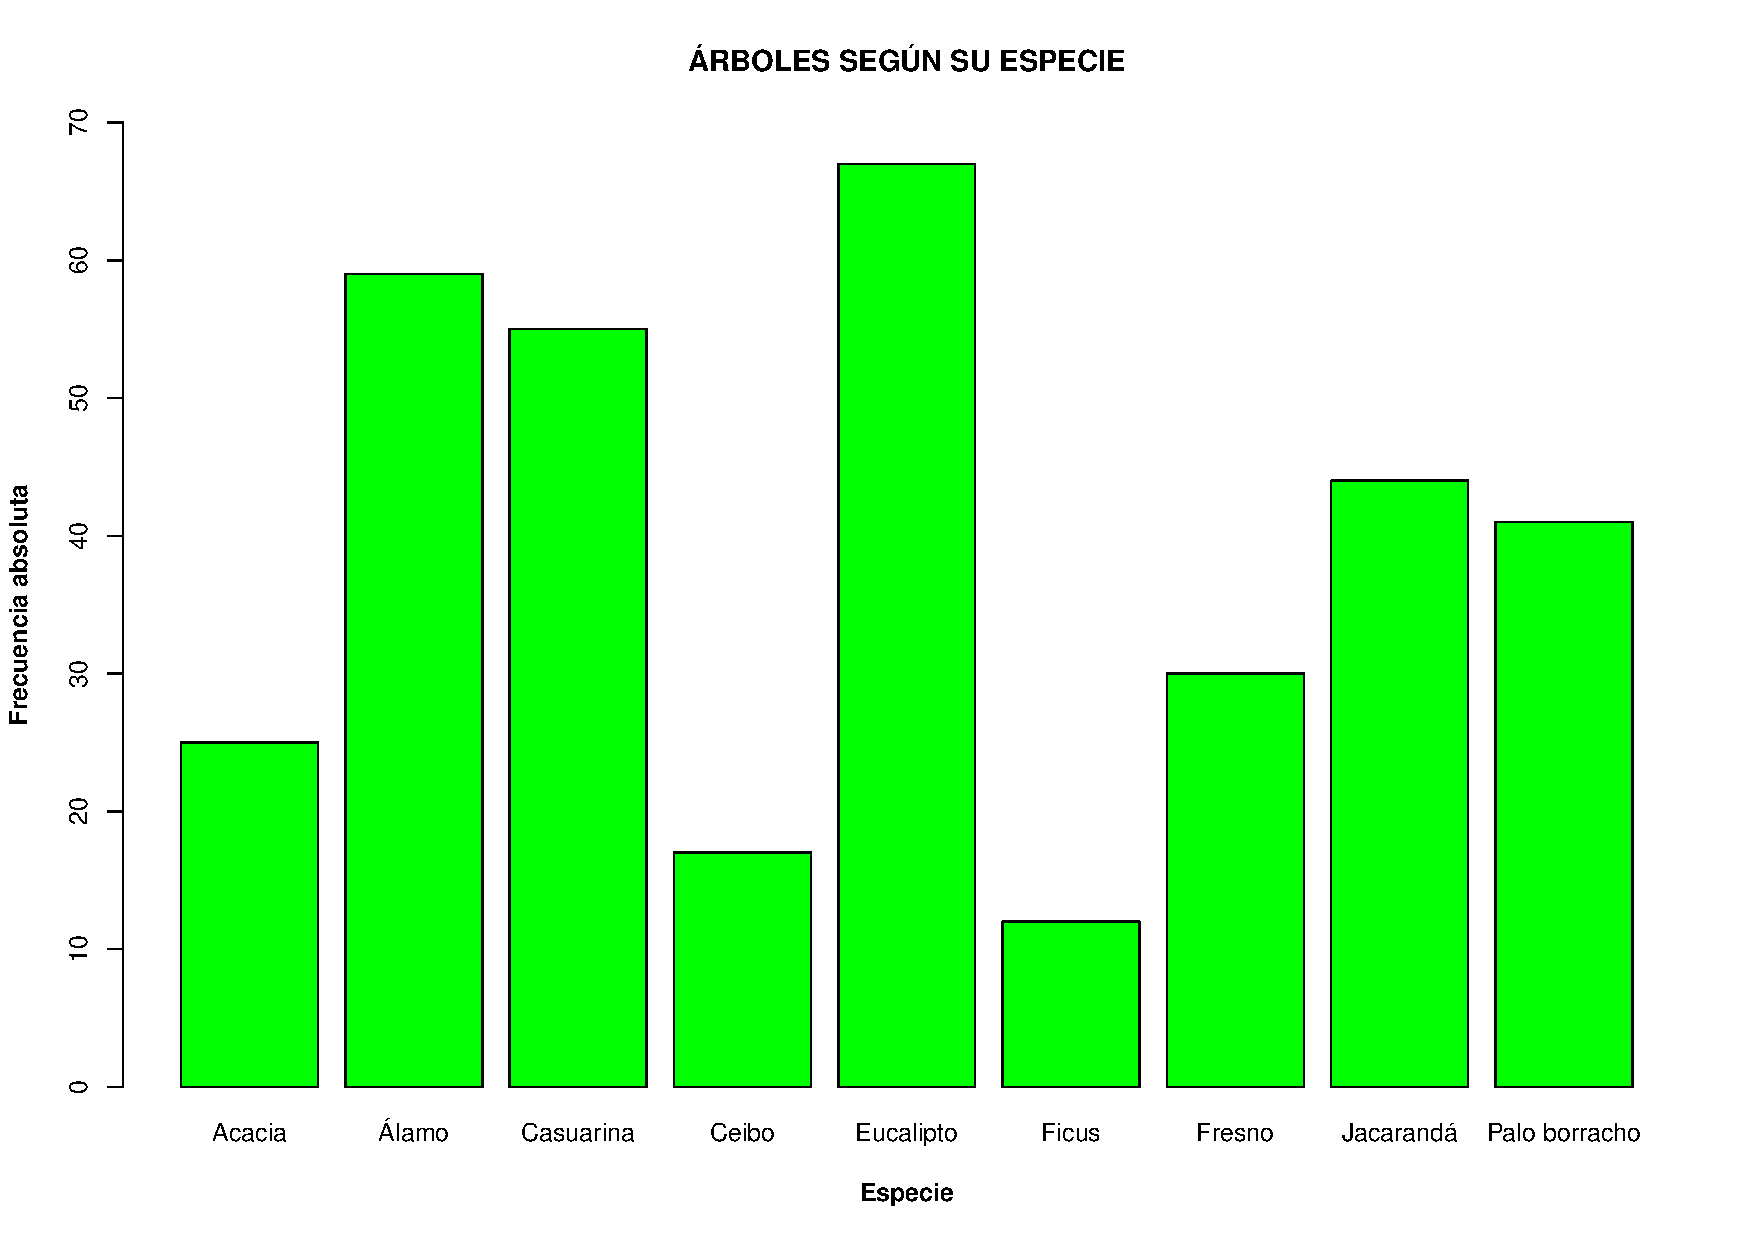
\includegraphics[width=0.9\linewidth]{barrasEspecie.pdf}
    \caption{Gráfico de barras.}
    \label{fig:barrasEspecie}
  \end{center}  
\end{figure}

\begin{justify}
  Si se observa el gráfico de la figura \ref{fig:barrasEspecie},
  se puede ver que la especie con más ejemplares en el censo resultó
  ser el eucalipto con una cantidad total de 67, seguido por Álamo
  con 59 y Casuarina con 55.
\end{justify}

% ============================================================================

\newpage
\subsection{Origen}

\begin{table}[h!]
  \begin{center}
    \begin{tabular}{| c | r | r |}
      \hline
      \textbf{Especie} & \textbf{Frecuencia absoluta} & \textbf{Frecuencia relativa} \\ \hline
      Exótico	& 241	& 0.6886 \\ \hline
      Nativo/Autóctono & 109 & 0.3114 \\ \hline
    \end{tabular}
    \caption{Tabla de frecuencias.}
    \label{tab:tablaOrigen}
  \end{center}
\end{table}

\begin{figure}[h!]
  \begin{center}
    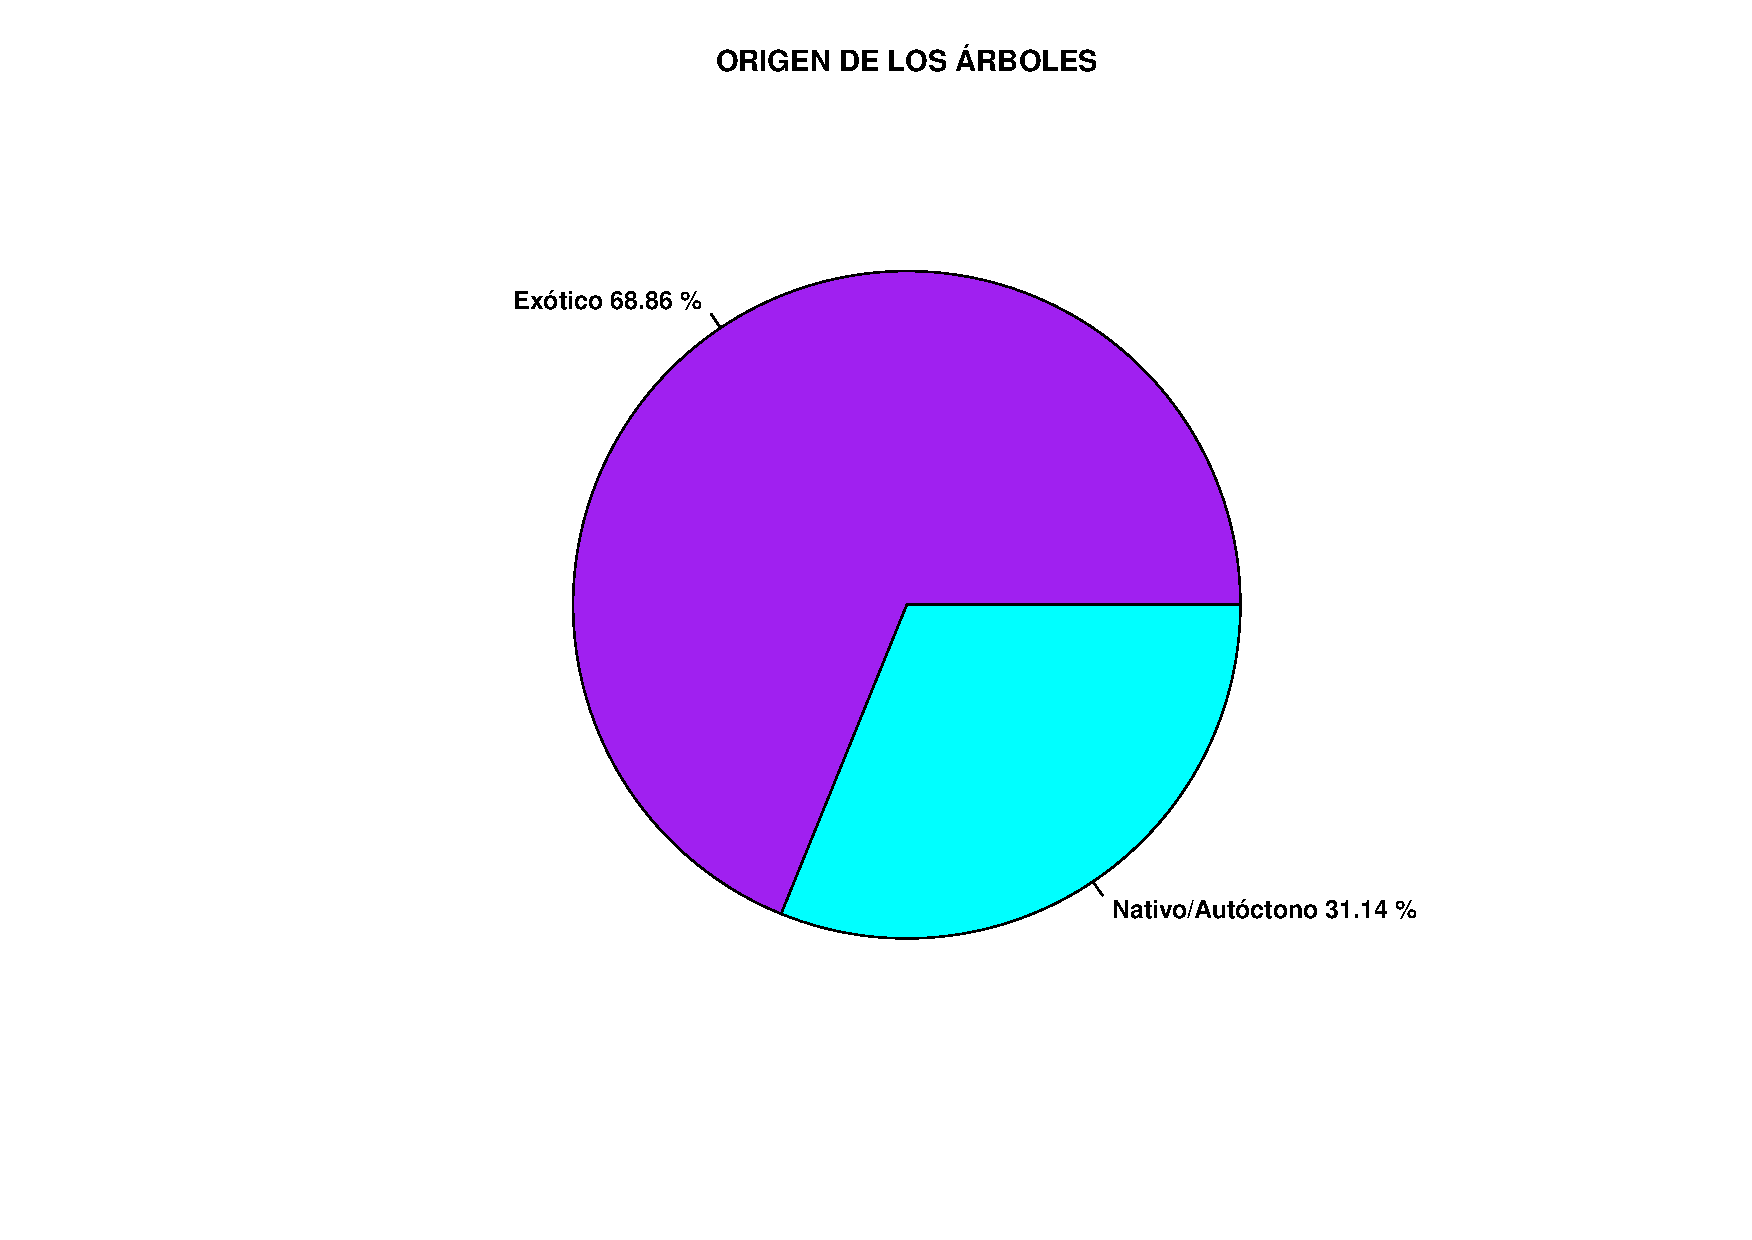
\includegraphics[width=0.9\linewidth]{pieOrigen.pdf}
    \caption{Gráfico de torta.}
    \label{fig:pieOrigen}
  \end{center}  
\end{figure}

\begin{justify}
  Observando la figura \ref{fig:pieOrigen} se puede ver que el 68.86\% de los
  árboles es de origen exótico y 31.14\% de origen Nativo/Autóctono.
\end{justify}

% ============================================================================

\newpage
\subsection{Brotes}

\begin{table}[h!]
  \begin{center}
    \begin{tabular}{| c | r | r | r | r |}
      \hline
      \multirow{3}{3cm}{\centering\textbf{Cantidad de brotes}} & 
      \multirow{3}{3cm}{\centering\textbf{Frecuencia absoluta}} & 
      \multirow{3}{3cm}{\centering\textbf{Frecuencia absoluta acumulada}} &
      \multirow{3}{3cm}{\centering\textbf{Frecuencia relativa}} & 
      \multirow{3}{3cm}{\centering\textbf{Frecuencia relativa acumulada}} \\
      & & & & \\
      & & & & \\ \hline
      1	& 1	& 1 & 0.0029	& 0.0029 \\ \hline
      1	& 16	& 17	& 0.0457	& 0.0486 \\ \hline
      2	& 65	& 82	& 0.1857	& 0.2343 \\ \hline
      3	& 100	& 182	& 0.2857	& 0.5200 \\ \hline
      4	& 87	& 269	& 0.2486	& 0.7686 \\ \hline
      5	& 47	& 316	& 0.1343	& 0.9029 \\ \hline
      6	& 25	& 341	& 0.0714	& 0.9743 \\ \hline
      7	& 7	& 348	& 0.0200	& 0.9943 \\ \hline
      8	& 2	& 350	& 0.0057	& 1.0000 \\ \hline
    \end{tabular}
    \caption{Tabla de frecuencias.}
    \label{tab:tablaBrotes}
  \end{center}
\end{table}

\begin{figure}[h!]
  \begin{center}
    \begin{subfigure}[b]{0.9\linewidth}
      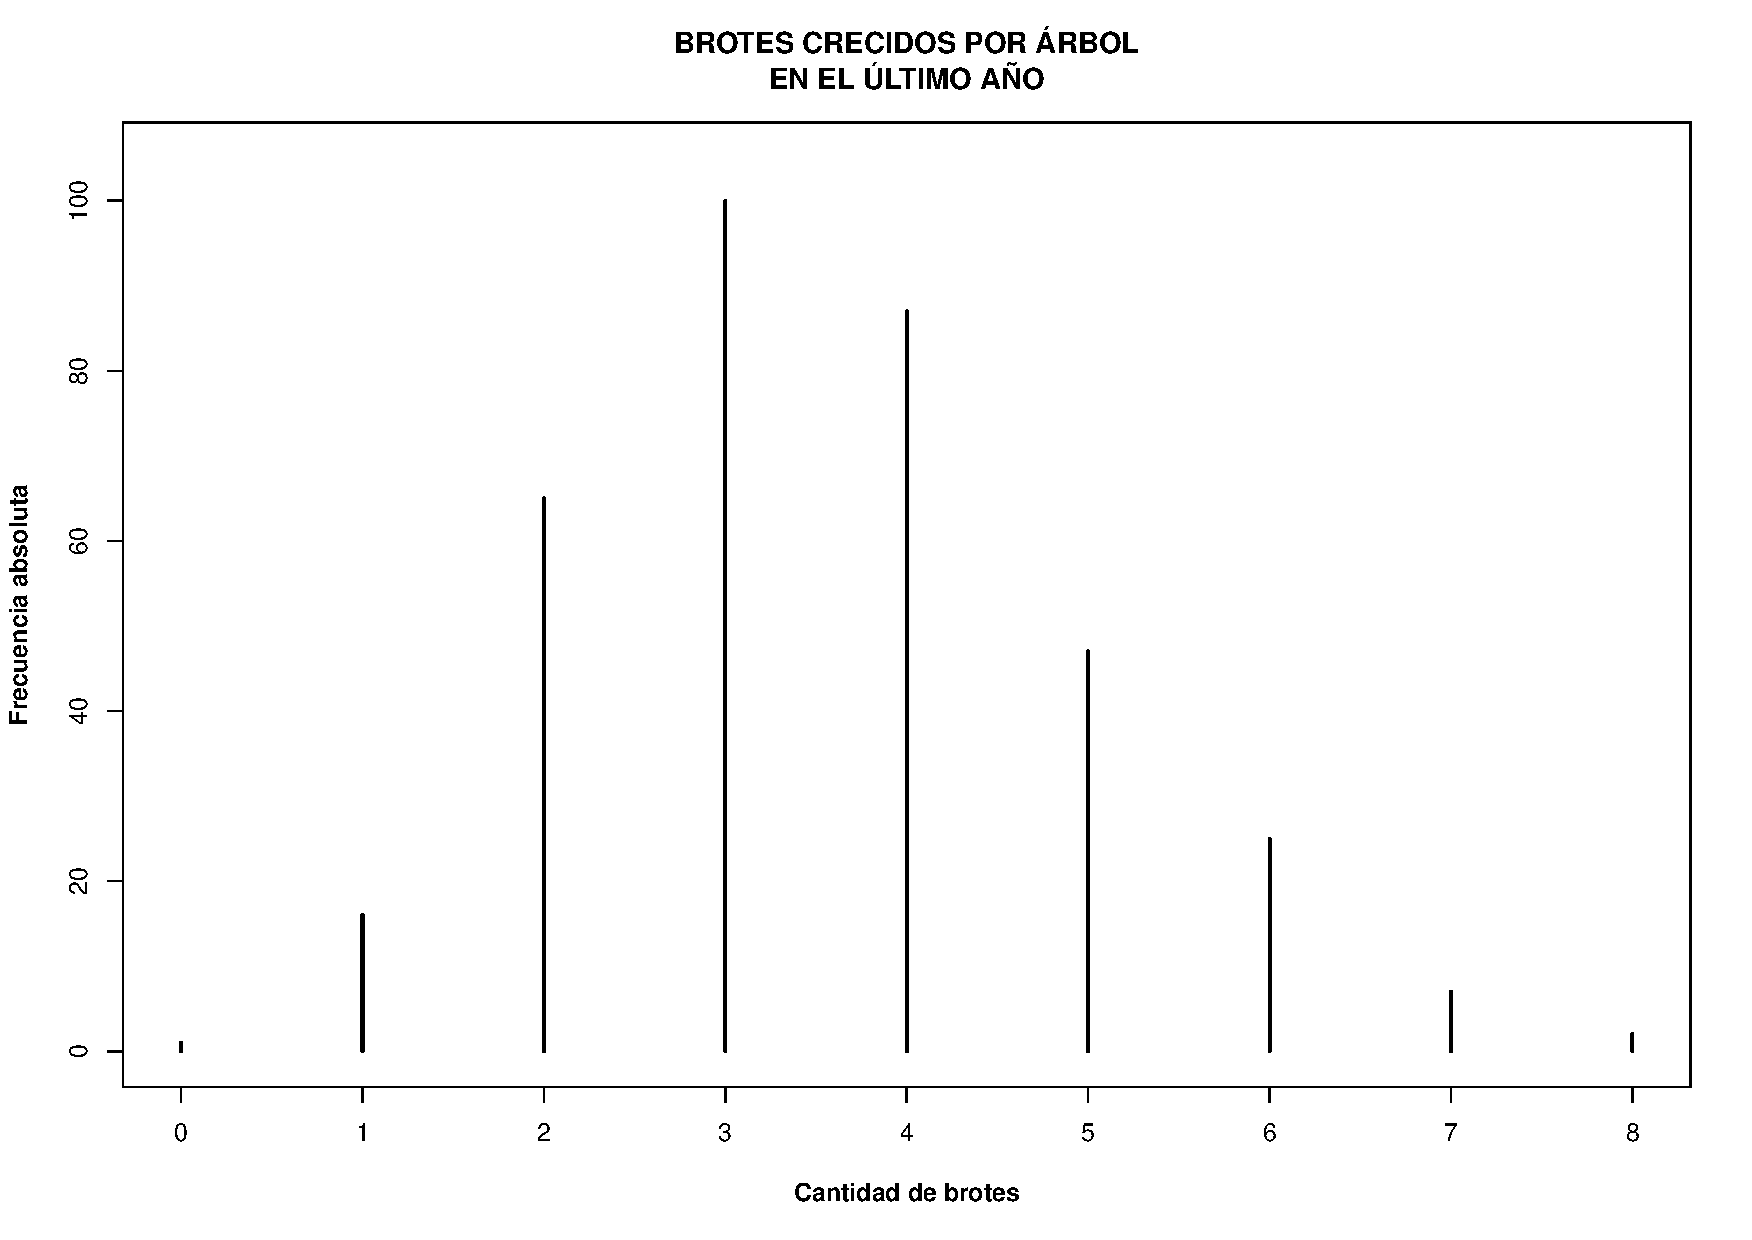
\includegraphics[width=\linewidth]{bastonesBrotes.pdf}
      \caption{Gráfico de bastones.}
      \label{fig:bastonesBrotes}
    \end{subfigure}
  \end{center}
\end{figure}

\begin{figure}[h!]
  \ContinuedFloat
  \begin{center}
    \begin{subfigure}[b]{0.9\linewidth}
      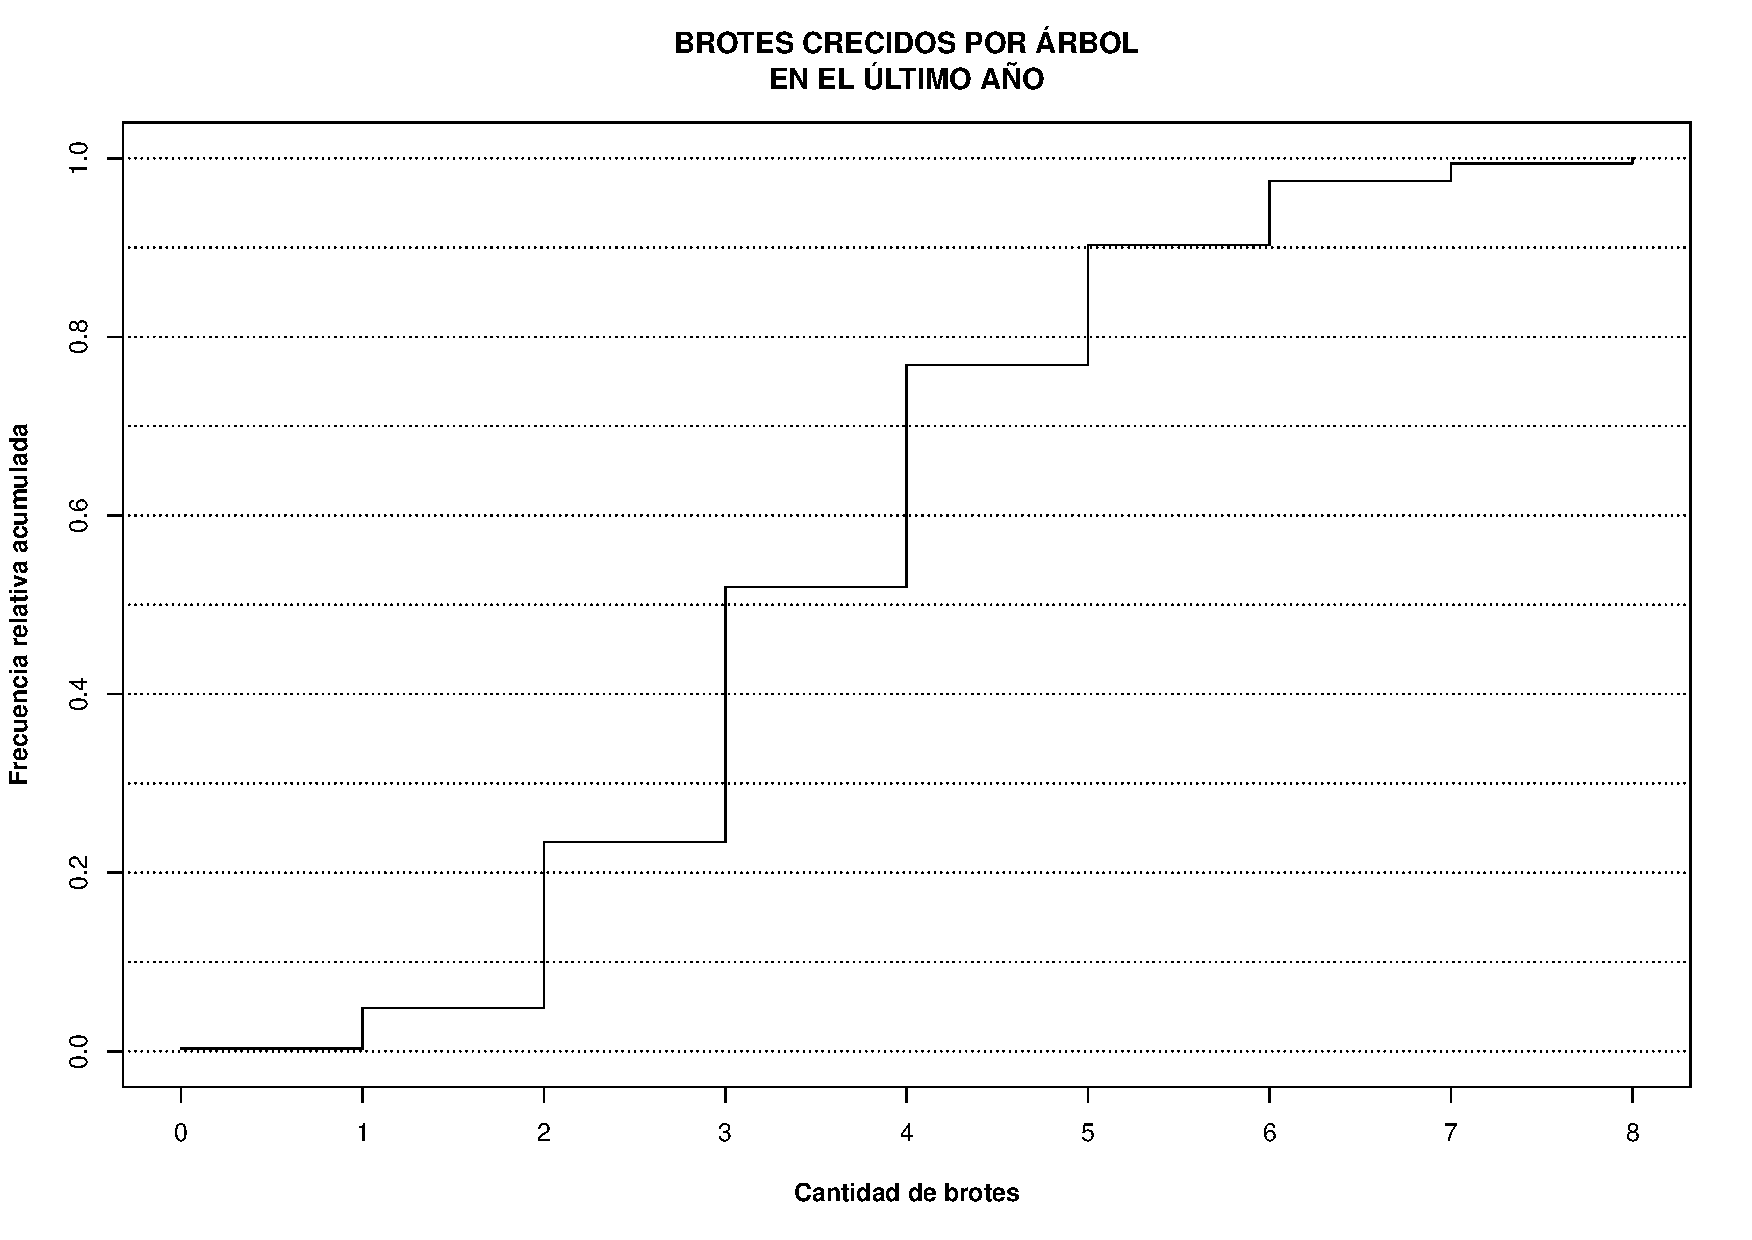
\includegraphics[width=\linewidth]{acumBrotes.pdf}
      \caption{Polígono acumulativo.}
      \label{fig:acumBrotes}
    \end{subfigure}
  \caption{}
  \end{center}  
\end{figure}

\newpage

\begin{justify}
  En el gráfico de la figura \ref{fig:bastonesBrotes} se observa que
  existe una mayor cantidad de árboles que presentaron 3 brotes crecidos
  durante el último año. La cantidad de brotes promedio resultó ser 3.5.
\end{justify}

% ============================================================================
% ============================================================================
% ============================================================================

\newpage
\section{Análisis bivariado}
\subsection{Origen/Especie}

\begin{table}[h!]
  \begin{center}
    \begin{tabular}{| c | r | r | r |}
      \hline
      \textbf{Especie} & \textbf{Exótico} & \textbf{Nativo/Autóctono} & \textbf{Total} \\ \hline
      Acacia & 18 & 7 & 25 \\ \hline
      Álamo & 59 & 0 & 59 \\ \hline
      Casuarina & 55 & 0 & 55 \\ \hline
      Ceibo & 0 & 17 & 17 \\ \hline
      Eucalipto & 67 & 0 & 67 \\ \hline
      Ficus & 12 & 0 & 12 \\ \hline
      Fresno & 30 & 0 & 30 \\ \hline
      Jacarandá & 0 & 44 & 44 \\ \hline
      Palo borracho & 0 & 41 & 41 \\ \hline
    \end{tabular}
    \caption{Tabla de frecuencias.}
    \label{tab:tablaOrigenEspecie}
  \end{center}
\end{table}

\begin{figure}[h!]
  \begin{center}
    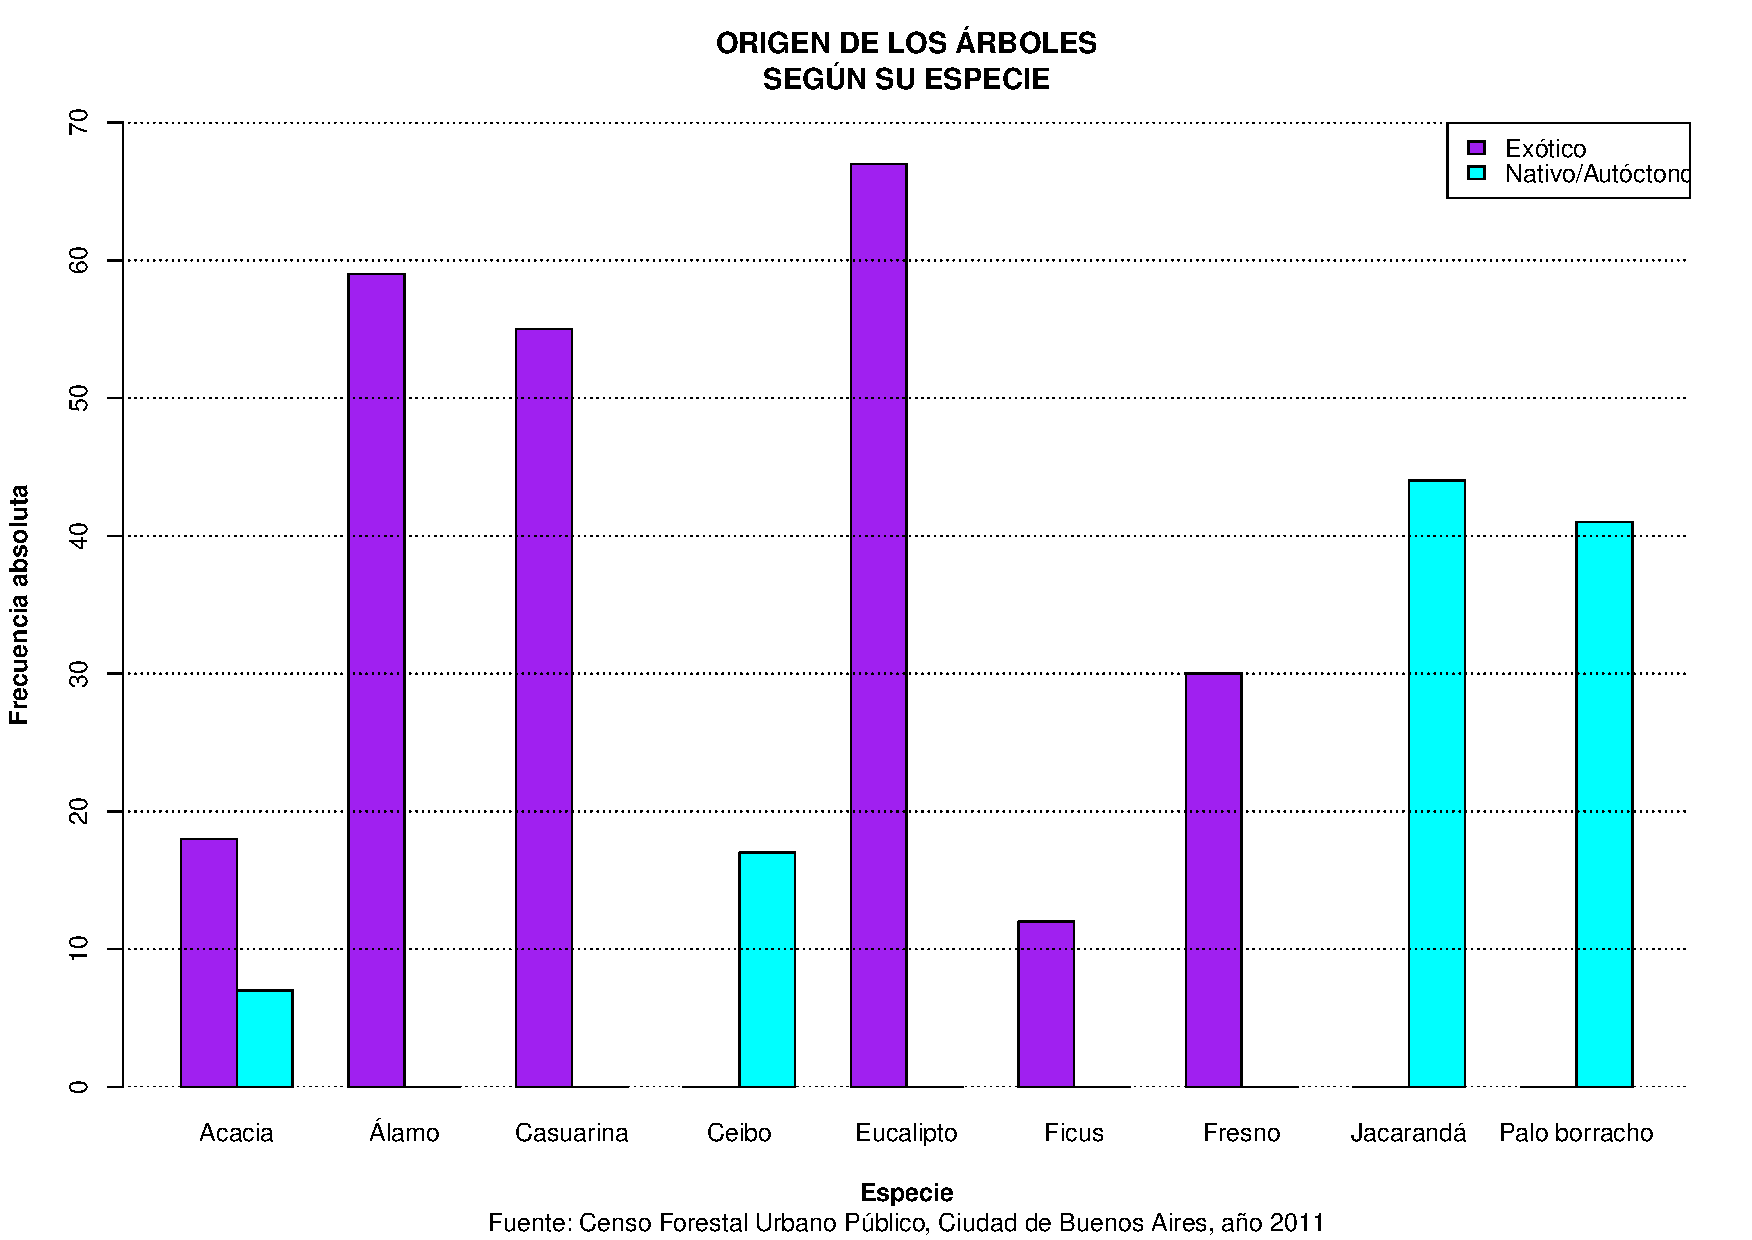
\includegraphics[width=0.9\linewidth]{barrasOrigenEspecie.pdf}
    \caption{Gráfico de barras.}
    \label{fig:barrasOrigenEspecie}
  \end{center}  
\end{figure}

\begin{justify}
  En la figura \ref{fig:barrasOrigenEspecie} se puede notar fácilmente
  las especies que son exclusivamente nativas o exóticas, excepto por la Acacia
  que es tanto nativa como exótica. La mayoria de las especies resultan ser
  de origen exótico.
\end{justify}

% ============================================================================

\newpage
\subsection{Brotes/Especie}

\begin{table}[h!]
  \begin{center}
    \begin{tabular}{| c | r |}
      \hline
      \textbf{Especie} & \textbf{Cantidad de brotes} \\ \hline
      Acacia & 93 \\ \hline
      Álamo & 156 \\ \hline
      Casuarina & 175 \\ \hline
      Ceibo & 78 \\ \hline
      Eucalipto & 194 \\ \hline
      Ficus & 31 \\ \hline
      Fresno & 91 \\ \hline
      Jacarandá & 230 \\ \hline
      Palo borracho & 196 \\ \hline
    \end{tabular}
  \caption{Tabla de frecuencias.}
  \label{tab:tablaBrotesEspecie}
  \end{center}
\end{table}

\begin{figure}[h!]
  \begin{center}
    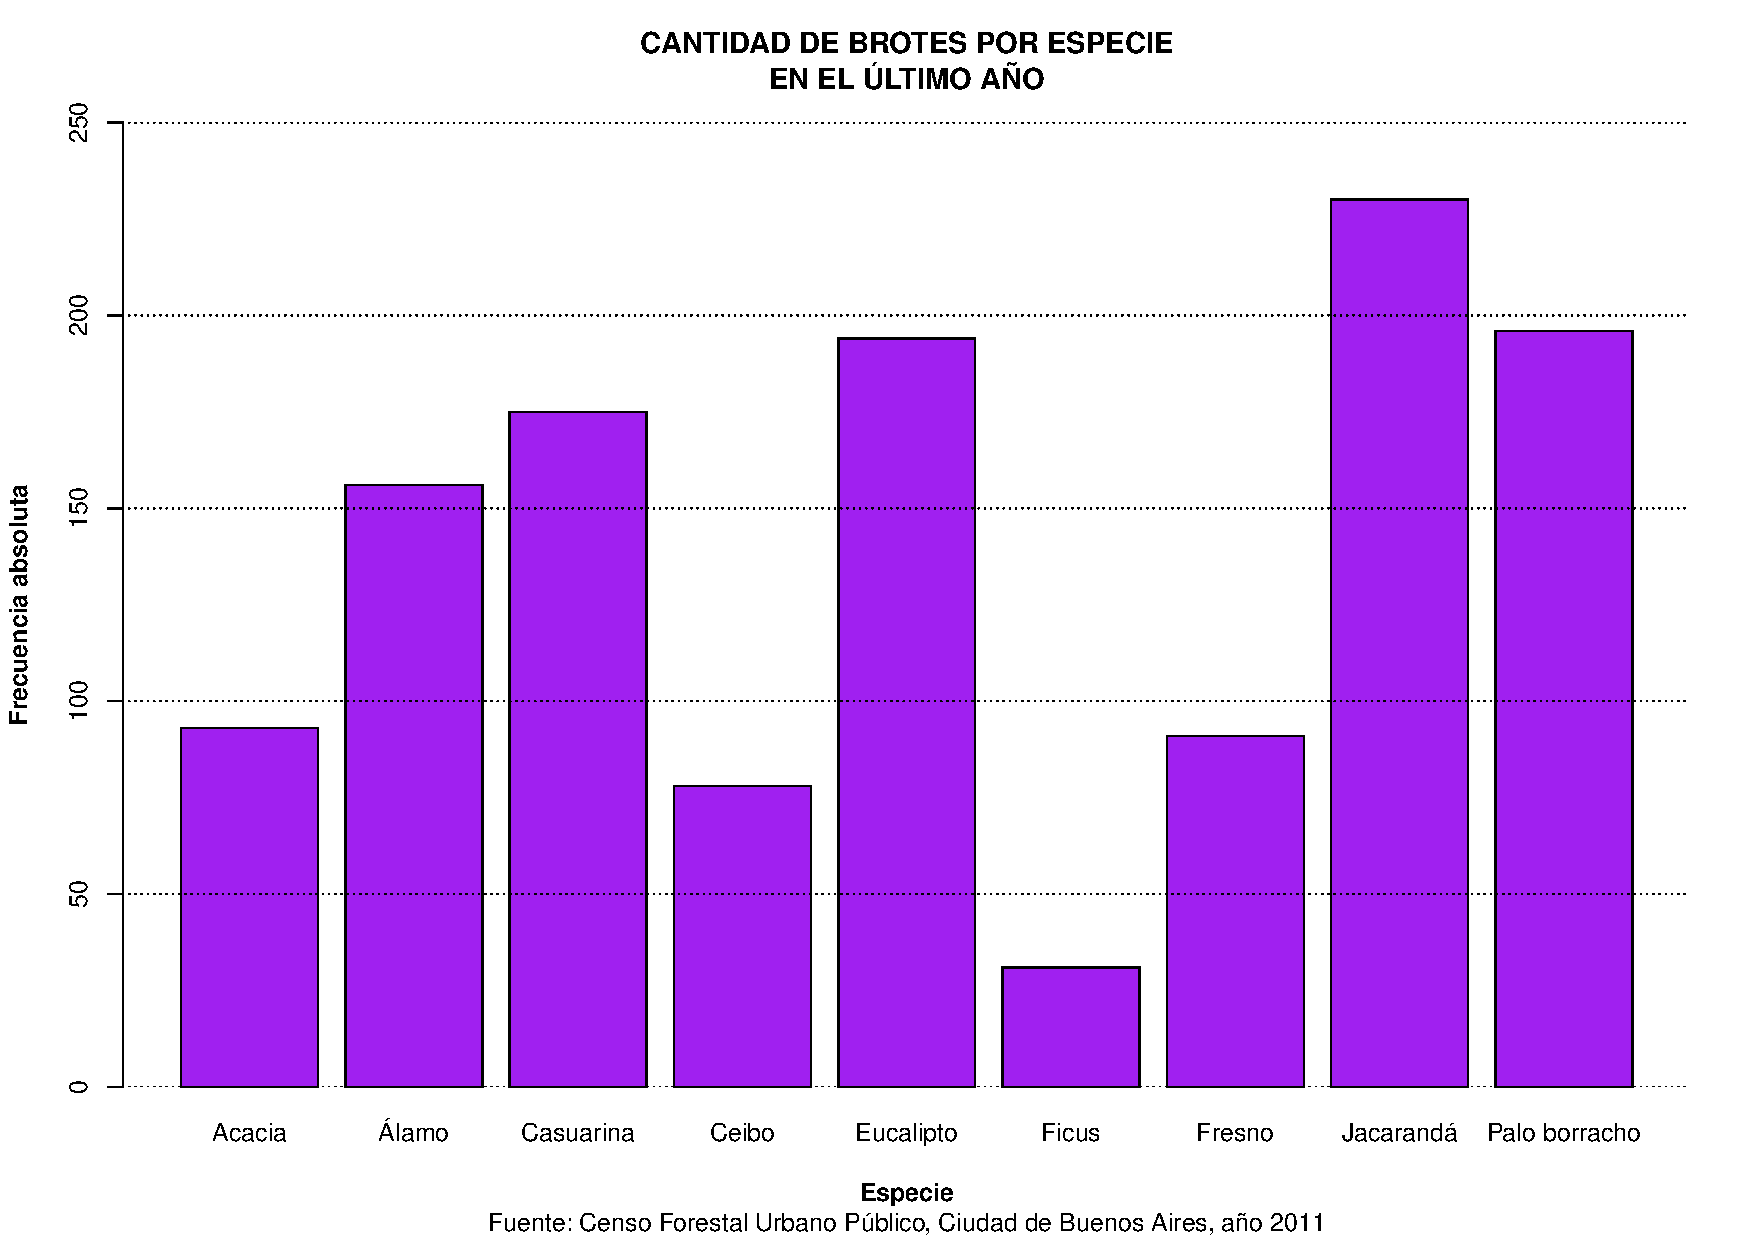
\includegraphics[width=0.9\linewidth]{barrasBrotesEspecie.pdf}
    \caption{Gráfico de barras.}
    \label{fig:barrasBrotesEspecie}
  \end{center}  
\end{figure}

\begin{justify}
  En el gráfico \ref{fig:barrasBrotesEspecie} se puede observar la cantidad
  de brotes que cada especie de árbol presentó durante el último año, siendo
  el Jacarandá la especie que mas brotes ha tenido.
\end{justify}

\end{document}